% Created 2019-02-14 Thu 14:59
% Intended LaTeX compiler: pdflatex
\documentclass[presentation]{beamer}
\usepackage[utf8]{inputenc}
\usepackage[T1]{fontenc}
\usepackage{graphicx}
\usepackage{grffile}
\usepackage{longtable}
\usepackage{wrapfig}
\usepackage{rotating}
\usepackage[normalem]{ulem}
\usepackage{amsmath}
\usepackage{textcomp}
\usepackage{amssymb}
\usepackage{capt-of}
\usepackage{hyperref}
\usepackage{awesomebox}
\usepackage{booktabs}
\usepackage{placeins}
\usepackage{siunitx}
\usepackage{minted}
\usetheme[progressbar=frametitle,block=fill]{metropolis}
\usetheme{default}
\author{\emph{Tejaswin Parthasarathy}, Mattia Gazzola}
\date{\today}
\title{Scientific computing in Python}
\subtitle{ME498: Comp. modeling \& optimization}
\hypersetup{
 pdfauthor={\emph{Tejaswin Parthasarathy}, Mattia Gazzola},
 pdftitle={Scientific computing in Python},
 pdfkeywords={},
 pdfsubject={},
 pdfcreator={Emacs 27.0.50 (Org mode 9.2)},
 pdflang={English}}
\begin{document}

\maketitle

\section{\texttt{numpy}}
\label{sec:orgc20d724}
\begin{frame}[label={sec:org7a10349},fragile]{\texttt{numpy} package \footnote{\href{https://www.numpy.org/}{numpy}}}
 \begin{itemize}
\item High-performance vector, matrix and higher-dimensional data structures for
\texttt{Python}
\item Shares a lot of similarity and differences (syntactically and semantically)
with \texttt{MATLAB} \footnote{\href{https://docs.scipy.org/doc/numpy/user/numpy-for-matlab-users.html}{numpy for Matlab users}}
\item Vectors, matrices and higher-dimensional data sets are \emph{(nd) arrays} in \texttt{numpy}
(there is also the \texttt{matrix} class, but it is being phased out)
\item Standard import---\texttt{import numpy as np}
\end{itemize}
\end{frame}
\begin{frame}[label={sec:org0adc71c},fragile]{Simple array creation in \texttt{numpy}}
 \note{:B\_note:
\begin{itemize}
\item Show the documentaion and how to browse it
\item Show as a demonstration\ldots{}
\end{itemize}}
\begin{itemize}
\item \texttt{v = np.array([1,2,3,4])} creates a vector (argument : list)
\item \texttt{M = np.array([[1, 2], [3, 4]])} creates a matrix (argument : nested list)
\item \texttt{type(v), type(M)} both return \texttt{numpy.ndarray}
\item The difference lies in the \alert{shape} seen using \texttt{v.shape/M.shape}\ldots{}
\item Alternatively use function \texttt{np.shape(v)}
\item Arrays can also have different data types, seen using \texttt{v.dtype}
\begin{itemize}
\item \texttt{npint32}, \texttt{np.float32}, \texttt{np.float64} (default)\ldots{}
\end{itemize}
\item \texttt{M = np.array([[1, 2], [3, 4]], dtype=int)}
\end{itemize}
\end{frame}
\begin{frame}[label={sec:org2539220},fragile]{Array generating functions}
 \note{:B\_note:
\begin{itemize}
\item Show as a demonstration\ldots{}
\end{itemize}}
\begin{itemize}
\item \texttt{v = np.arange(0,11,2)} gives ranges similar to \texttt{Python's range}
\item \texttt{v = np.arange(0, 11, 0.1)} is also valid! (gives step of 0.1)
\item \texttt{v = np.linspace(0, 1, 3)} creates a linearly spaced vector [0, 0.5, 1.]
\item Also have \texttt{logspace, geomspace} for other progressions
\item Multidimensional array creation using \texttt{meshgrid, ndgrid} and others
\item Other useful ones are \texttt{ones} (which generates matrix with all 1), \texttt{zeros}
(simliar) and \texttt{eye} (identity matrix)
\end{itemize}
\end{frame}

\begin{frame}[label={sec:org0ae008d},fragile]{Random numbers}
 \note{:B\_note:
\begin{itemize}
\item Show as a demonstration
\item np.random.rand(5,5)\ldots{}same syntax for randn too..
\item np.random.randint(1,5,size=(2,4))
\end{itemize}}
\begin{itemize}
\item We'll work extensively with random numbers, so let's see what \texttt{numpy} has
to offer
\item \texttt{np.random.rand(<shape>)} gives random floats from uniform dist. in [0, 1)
\item \texttt{np.random.randn(<shape>)} gives random floats from univariate normal
dist. with \(\mu = 0\) and \(\sigma = 1\)
\item \texttt{np.random.randint(low, high, size)} gives random ints from discrete uniform dist.
in \texttt{[low, high)}
\end{itemize}
\end{frame}
\begin{frame}[label={sec:orgb7c7d58},fragile]{Indexing}
 \note{:B\_note:
\begin{itemize}
\item Show as a demonstration of all
\item A = np.random.randn(5,5); A[2:3,:] is slicing
\item Fancy indexing: idx\_rows = [1,5]; idx\_cols = [1,2,4]; A[idx\_rows, idx\_cols]
\item mask\_row = [True, False, False, False, True]; A[mask\_row]. Compare with
A[idx\_rows, :] above
\end{itemize}}
\begin{itemize}
\item Slicing works for \texttt{numpy} arrays too, across any dimension!
\item Fancy indexing
\begin{itemize}
\item Extends slicing to be more useful + practical
\end{itemize}
\item Masking
\begin{itemize}
\item Bools to \emph{mask} what is not necessary
\item Useful with conditional functions (e.g. \texttt{x < 5})
\end{itemize}
\item Reshaping using \texttt{np.reshape} changes index access
\end{itemize}
\end{frame}

\begin{frame}[label={sec:org3411e3d},fragile]{Linear Algebra}
 \note{:B\_note:
\begin{itemize}
\item In the demo construct structure A with 1:25 using \texttt{A =
      np.linspace(1.0,25.0,25)} and then do \texttt{A = A.reshape(5,5)}
\item Use \texttt{np.arange} for constructing \texttt{v=np.arange(0, 5)}
\item Show that \texttt{A*v} does element wise onlt
\end{itemize}}

\begin{itemize}
\item Scalar operations on an array \texttt{A}
\begin{itemize}
\item \texttt{A + 2}, \texttt{A * 2} , \texttt{A ** 2} \ldots{}
\end{itemize}
\item Element wise operations on an array \texttt{A}
\begin{itemize}
\item \texttt{A * A}, \texttt{A / A} \ldots{}
\item What do you get when you do \texttt{A*v}? \alert{DEMO}
\end{itemize}
\item Matrix algebra on an array \texttt{A}
\begin{itemize}
\item \texttt{np.dot(A, v)} or \texttt{A.dot(v)} or simply \texttt{A@v}
\item Shape needs to be compliant! \texttt{numpy} also has broadcasts that is useful,
but is confusing and so is not covered here \ldots{}
\end{itemize}
\end{itemize}
\end{frame}

\begin{frame}[label={sec:org0d84c63},fragile]{Practice}
 \begin{block}{Please attempt}
\begin{itemize}
\item \texttt{12\_numpy\_library.ipynb}
\item For a more extensive tutorial: \url{https://github.com/donnemartin/data-science-ipython-notebooks\#numpy}
\end{itemize}
\end{block}
\end{frame}
\note{:B\_note:
\begin{itemize}
\item Access to \url{https://github.com/donnemartin/data-science-ipython-notebooks}
especially the numpy section
\end{itemize}}

\section{Genetic algorithm using \texttt{numpy}}
\label{sec:org7d2850c}
\begin{frame}[label={sec:org6cbe02f}]{Schematic}
\footnotesize
\begin{figure}[htbp]
\centering
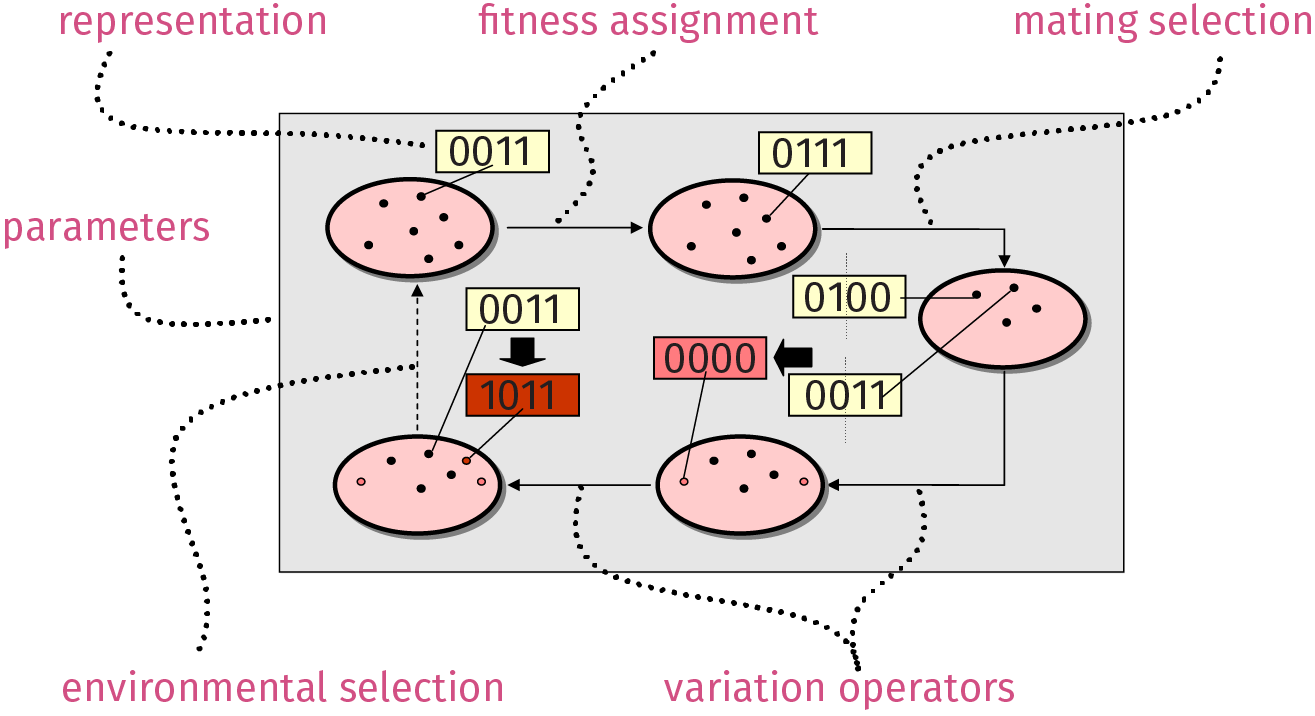
\includegraphics[width=1.0\textwidth]{images/ga_schematic.png}
\caption{Schematic of an evolutionary search algorithm}
\end{figure}
\end{frame}
\begin{frame}[label={sec:orga6d8564}]{Let's use GA to solve\ldots{}}
\begin{block}{Problem statement}
Maximize the function \(f(\mathbf{x}) = \sum_{i=1}^{6} w_i x_i\) for a given
set of weights \(w_i\), with the constraints that \(x_i \; \in \; [-4,4] \;
   \forall \; i\).

\(\therefore\) Domain \(\mathbb{D}\) of the search is \(\mathbb{D}:= [-4,4]^6\).

Optimization problem: \(\left(\mathbb{D}, \mathbb{R} , \mathbf{f}, \geq \right)\).
\end{block}
\end{frame}
\begin{frame}[label={sec:orgeb346c1},fragile]{Representation?}
 \begin{block}{Bitvector? Float vector?}
Pick a representation for \(\mathbf{x}\)
\end{block}
In any case, \texttt{np.array} seems useful. You can make a bitvector using
\texttt{np.array(..., dtype=bool)}
\end{frame}
\begin{frame}[label={sec:org9a024f8},fragile]{GA parameters}
 \begin{block}{Decisions}
\begin{itemize}
\item How long are you going to run your campaign? (Number of generations)
\item How many solutions will you consider in one step? (Population size)
\begin{itemize}
\item If so, whats your degree of freedom? (How many numbers should you change)
\end{itemize}
\end{itemize}
\end{block}
All these are just floating point numbers

\begin{block}{Initialization}
\begin{itemize}
\item How will you initialize your population?
\end{itemize}
\end{block}

Consider the \texttt{np.random} module\ldots{}
\end{frame}

\begin{frame}[label={sec:orgf3488d5}]{Fitness assignment}
\begin{block}{What's your fitness?}
\begin{itemize}
\item Feed in objective function directly?
\item Competitive fitness between members?
\end{itemize}
\end{block}
Use matrix-vector products and/or slicing to determine fitness
\end{frame}
\begin{frame}[label={sec:orga6bd0b3},fragile]{Selection (for variation)}
 \begin{block}{Stochastic / Deterministic}
\begin{itemize}
\item How many parents do you want to select? Or do you want to leave it up to
the algorithm?
\item Deterministic / Stochastic?
\begin{itemize}
\item Remember that stochastic selection is usally used for variation, but
we do not need to do it necessarily\ldots{}
\end{itemize}
\item Competitive fitness between members?
\begin{itemize}
\item It's definitely a good exercise to learn \texttt{numpy}
\end{itemize}
\end{itemize}
\end{block}
\texttt{np.argsort/np.sort} is very useful to sort/rank stuff, indexing magic
needed. The brave souls doing SUS may also need \texttt{searchsorted, cumsum, sum}
and so on (familiarize yourself with the \texttt{numpy} documentation)
\end{frame}
\begin{frame}[label={sec:orga084e3a},fragile]{Variation}
 \begin{block}{Recombination}
\begin{itemize}
\item What will be your \(p_c\), the rate of recombination?
\item Is there a limit on the number of offspring you generate?
\item How to achieve crossover for your representation?
\item Uniform crossover? N-point crossover? \ldots{}
\item In which gene do you want to effect crossover?
\end{itemize}
\end{block}
Extensively use slicing and index magic. You may use any algorithm (say
using the \texttt{\%} operator) to select parents.
\end{frame}
\begin{frame}[label={sec:org6ad5101},fragile]{Variation}
 \begin{block}{Mutation}
\begin{itemize}
\item What will be your \(p_m\), the rate of mutation?
\item How do you want to achieve mutation? Flip bits? Number exchange? Random numbers?
\item Do you want to mutate the entire vector? Or only one gene?
\end{itemize}
\end{block}
\texttt{np.random} once again. You can also use other \texttt{np} tools
\end{frame}
\begin{frame}[label={sec:org8e036a9}]{Selection (environmental)}
\begin{block}{Constraints / Deterministic schemes}
\begin{itemize}
\item What about constraints of \(-4 \leq x_i \leq 4\)?
\item How do you select individuals (chromosomes) from the population to
propogate to the next generation? Objective function alone?
\item If so what scheme do you want to use? \(\left( \mu, \lambda \right)\),
\(\left( \mu + \lambda \right)\),\ldots{}?
\end{itemize}
\end{block}
All the tools seen above apply to this case too\ldots{}
\end{frame}
\begin{frame}[label={sec:org2514b38}]{Putting it all together}
\begin{block}{Convergence, performance, diagnostics}
\begin{itemize}
\item Now that we have all the \emph{modules}, how do they perform when you put
them together?
\item How do we track performance as generations progress?
\item Can you think of some diagnostics that may well-characterize the scheme
that you have just developed?
\end{itemize}
\end{block}
\end{frame}
\begin{frame}[label={sec:org444b6d5}]{Practice}
\begin{block}{Exploration}
\begin{itemize}
\item Explore representations, parameters and all other design choices that you
made
\item You will essentially be doing a scaled up version of this exercise for
your project 1
\end{itemize}
\end{block}
\end{frame}
\end{document}
